\documentclass[1p]{elsarticle_modified}
%\bibliographystyle{elsarticle-num}

%\usepackage[colorlinks]{hyperref}
%\usepackage{abbrmath_seonhwa} %\Abb, \Ascr, \Acal ,\Abf, \Afrak
\usepackage{amsfonts}
\usepackage{amssymb}
\usepackage{amsmath}
\usepackage{amsthm}
\usepackage{scalefnt}
\usepackage{amsbsy}
\usepackage{kotex}
\usepackage{caption}
\usepackage{subfig}
\usepackage{color}
\usepackage{graphicx}
\usepackage{xcolor} %% white, black, red, green, blue, cyan, magenta, yellow
\usepackage{float}
\usepackage{setspace}
\usepackage{hyperref}

\usepackage{tikz}
\usetikzlibrary{arrows}

\usepackage{multirow}
\usepackage{array} % fixed length table
\usepackage{hhline}

%%%%%%%%%%%%%%%%%%%%%
\makeatletter
\renewcommand*\env@matrix[1][\arraystretch]{%
	\edef\arraystretch{#1}%
	\hskip -\arraycolsep
	\let\@ifnextchar\new@ifnextchar
	\array{*\c@MaxMatrixCols c}}
\makeatother %https://tex.stackexchange.com/questions/14071/how-can-i-increase-the-line-spacing-in-a-matrix
%%%%%%%%%%%%%%%

\usepackage[normalem]{ulem}

\newcommand{\msout}[1]{\ifmmode\text{\sout{\ensuremath{#1}}}\else\sout{#1}\fi}
%SOURCE: \msout is \stkout macro in https://tex.stackexchange.com/questions/20609/strikeout-in-math-mode

\newcommand{\cancel}[1]{
	\ifmmode
	{\color{red}\msout{#1}}
	\else
	{\color{red}\sout{#1}}
	\fi
}

\newcommand{\add}[1]{
	{\color{blue}\uwave{#1}}
}

\newcommand{\replace}[2]{
	\ifmmode
	{\color{red}\msout{#1}}{\color{blue}\uwave{#2}}
	\else
	{\color{red}\sout{#1}}{\color{blue}\uwave{#2}}
	\fi
}

\newcommand{\Sol}{\mathcal{S}} %segment
\newcommand{\D}{D} %diagram
\newcommand{\A}{\mathcal{A}} %arc


%%%%%%%%%%%%%%%%%%%%%%%%%%%%%5 test

\def\sl{\operatorname{\textup{SL}}(2,\Cbb)}
\def\psl{\operatorname{\textup{PSL}}(2,\Cbb)}
\def\quan{\mkern 1mu \triangleright \mkern 1mu}

\theoremstyle{definition}
\newtheorem{thm}{Theorem}[section]
\newtheorem{prop}[thm]{Proposition}
\newtheorem{lem}[thm]{Lemma}
\newtheorem{ques}[thm]{Question}
\newtheorem{cor}[thm]{Corollary}
\newtheorem{defn}[thm]{Definition}
\newtheorem{exam}[thm]{Example}
\newtheorem{rmk}[thm]{Remark}
\newtheorem{alg}[thm]{Algorithm}

\newcommand{\I}{\sqrt{-1}}
\begin{document}

%\begin{frontmatter}
%
%\title{Boundary parabolic representations of knots up to 8 crossings}
%
%%% Group authors per affiliation:
%\author{Yunhi Cho} 
%\address{Department of Mathematics, University of Seoul, Seoul, Korea}
%\ead{yhcho@uos.ac.kr}
%
%
%\author{Seonhwa Kim} %\fnref{s_kim}}
%\address{Center for Geometry and Physics, Institute for Basic Science, Pohang, 37673, Korea}
%\ead{ryeona17@ibs.re.kr}
%
%\author{Hyuk Kim}
%\address{Department of Mathematical Sciences, Seoul National University, Seoul 08826, Korea}
%\ead{hyukkim@snu.ac.kr}
%
%\author{Seokbeom Yoon}
%\address{Department of Mathematical Sciences, Seoul National University, Seoul, 08826,  Korea}
%\ead{sbyoon15@snu.ac.kr}
%
%\begin{abstract}
%We find all boundary parabolic representation of knots up to 8 crossings.
%
%\end{abstract}
%\begin{keyword}
%    \MSC[2010] 57M25 
%\end{keyword}
%
%\end{frontmatter}

%\linenumbers
%\tableofcontents
%
\newcommand\colored[1]{\textcolor{white}{\rule[-0.35ex]{0.8em}{1.4ex}}\kern-0.8em\color{red} #1}%
%\newcommand\colored[1]{\textcolor{white}{ #1}\kern-2.17ex	\textcolor{white}{ #1}\kern-1.81ex	\textcolor{white}{ #1}\kern-2.15ex\color{red}#1	}

{\Large $\underline{12a_{0027}~(K12a_{0027})}$}

\setlength{\tabcolsep}{10pt}
\renewcommand{\arraystretch}{1.6}
\vspace{1cm}\begin{tabular}{m{100pt}>{\centering\arraybackslash}m{274pt}}
\multirow{5}{120pt}{
	\centering
	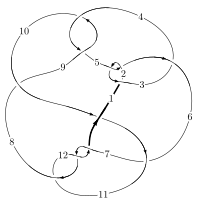
\includegraphics[width=112pt]{../../../GIT/diagram.site/Diagrams/png/828_12a_0027.png}\\
\ \ \ A knot diagram\footnotemark}&
\allowdisplaybreaks
\textbf{Linearized knot diagam} \\
\cline{2-2}
 &
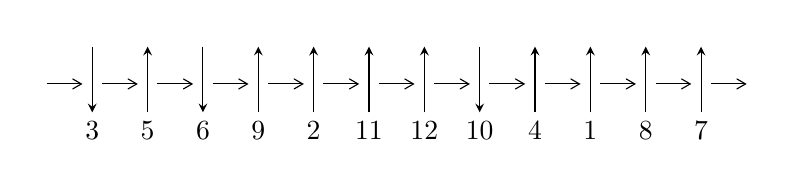
\begin{tikzpicture}[x=20pt, y=17pt]
	% nodes
	\node (C0) at (0, 0) {};
	\node (C1) at (1, 0) {};
	\node (C1U) at (1, +1) {};
	\node (C1D) at (1, -1) {3};

	\node (C2) at (2, 0) {};
	\node (C2U) at (2, +1) {};
	\node (C2D) at (2, -1) {5};

	\node (C3) at (3, 0) {};
	\node (C3U) at (3, +1) {};
	\node (C3D) at (3, -1) {6};

	\node (C4) at (4, 0) {};
	\node (C4U) at (4, +1) {};
	\node (C4D) at (4, -1) {9};

	\node (C5) at (5, 0) {};
	\node (C5U) at (5, +1) {};
	\node (C5D) at (5, -1) {2};

	\node (C6) at (6, 0) {};
	\node (C6U) at (6, +1) {};
	\node (C6D) at (6, -1) {11};

	\node (C7) at (7, 0) {};
	\node (C7U) at (7, +1) {};
	\node (C7D) at (7, -1) {12};

	\node (C8) at (8, 0) {};
	\node (C8U) at (8, +1) {};
	\node (C8D) at (8, -1) {10};

	\node (C9) at (9, 0) {};
	\node (C9U) at (9, +1) {};
	\node (C9D) at (9, -1) {4};

	\node (C10) at (10, 0) {};
	\node (C10U) at (10, +1) {};
	\node (C10D) at (10, -1) {1};

	\node (C11) at (11, 0) {};
	\node (C11U) at (11, +1) {};
	\node (C11D) at (11, -1) {8};

	\node (C12) at (12, 0) {};
	\node (C12U) at (12, +1) {};
	\node (C12D) at (12, -1) {7};
	\node (C13) at (13, 0) {};

	% arrows
	\draw[->,>={angle 60}]
	(C0) edge (C1) (C1) edge (C2) (C2) edge (C3) (C3) edge (C4) (C4) edge (C5) (C5) edge (C6) (C6) edge (C7) (C7) edge (C8) (C8) edge (C9) (C9) edge (C10) (C10) edge (C11) (C11) edge (C12) (C12) edge (C13) ;	\draw[->,>=stealth]
	(C1U) edge (C1D) (C2D) edge (C2U) (C3U) edge (C3D) (C4D) edge (C4U) (C5D) edge (C5U) (C6D) edge (C6U) (C7D) edge (C7U) (C8U) edge (C8D) (C9D) edge (C9U) (C10D) edge (C10U) (C11D) edge (C11U) (C12D) edge (C12U) ;
	\end{tikzpicture} \\
\hhline{~~} \\& 
\textbf{Solving Sequence} \\ \cline{2-2} 
 &
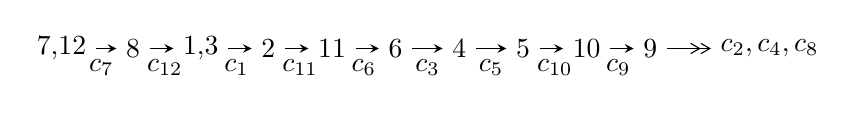
\begin{tikzpicture}[x=23pt, y=7pt]
	% node
	\node (A0) at (-1/8, 0) {7,12};
	\node (A1) at (1, 0) {8};
	\node (A2) at (33/16, 0) {1,3};
	\node (A3) at (25/8, 0) {2};
	\node (A4) at (33/8, 0) {11};
	\node (A5) at (41/8, 0) {6};
	\node (A6) at (49/8, 0) {4};
	\node (A7) at (57/8, 0) {5};
	\node (A8) at (65/8, 0) {10};
	\node (A9) at (73/8, 0) {9};
	\node (C1) at (1/2, -1) {$c_{7}$};
	\node (C2) at (3/2, -1) {$c_{12}$};
	\node (C3) at (21/8, -1) {$c_{1}$};
	\node (C4) at (29/8, -1) {$c_{11}$};
	\node (C5) at (37/8, -1) {$c_{6}$};
	\node (C6) at (45/8, -1) {$c_{3}$};
	\node (C7) at (53/8, -1) {$c_{5}$};
	\node (C8) at (61/8, -1) {$c_{10}$};
	\node (C9) at (69/8, -1) {$c_{9}$};
	\node (A10) at (11, 0) {$c_{2},c_{4},c_{8}$};

	% edge
	\draw[->,>=stealth]	
	(A0) edge (A1) (A1) edge (A2) (A2) edge (A3) (A3) edge (A4) (A4) edge (A5) (A5) edge (A6) (A6) edge (A7) (A7) edge (A8) (A8) edge (A9) ;
	\draw[->>,>={angle 60}]	
	(A9) edge (A10);
\end{tikzpicture} \\ 

\end{tabular} \\

\footnotetext{
The image of knot diagram is generated by the software ``\textbf{Draw programme}" developed by Andrew Bartholomew(\url{http://www.layer8.co.uk/maths/draw/index.htm\#Running-draw}), where we modified some parts for our purpose(\url{https://github.com/CATsTAILs/LinksPainter}).
}\phantom \\ \newline 
\centering \textbf{Ideals for irreducible components\footnotemark of $X_{\text{par}}$} 
 
\begin{align*}
I^u_{1}&=\langle 
7 u^{98}-14 u^{97}+\cdots+2 b-3,\;-2 u^{98}+6 u^{97}+\cdots+2 a+13,\;u^{99}-3 u^{98}+\cdots-5 u+1\rangle \\
I^u_{2}&=\langle 
u^2 a+b+a,\;- u^2 a+a^2- a u- a- u,\;u^3+u^2+2 u+1\rangle \\
\\
\end{align*}
\raggedright * 2 irreducible components of $\dim_{\mathbb{C}}=0$, with total 105 representations.\\
\footnotetext{All coefficients of polynomials are rational numbers. But the coefficients are sometimes approximated in decimal forms when there is not enough margin.}
\newpage
\renewcommand{\arraystretch}{1}
\centering \section*{I. $I^u_{1}= \langle 7 u^{98}-14 u^{97}+\cdots+2 b-3,\;-2 u^{98}+6 u^{97}+\cdots+2 a+13,\;u^{99}-3 u^{98}+\cdots-5 u+1 \rangle$}
\flushleft \textbf{(i) Arc colorings}\\
\begin{tabular}{m{7pt} m{180pt} m{7pt} m{180pt} }
\flushright $a_{7}=$&$\begin{pmatrix}1\\0\end{pmatrix}$ \\
\flushright $a_{12}=$&$\begin{pmatrix}0\\u\end{pmatrix}$ \\
\flushright $a_{8}=$&$\begin{pmatrix}1\\- u^2\end{pmatrix}$ \\
\flushright $a_{1}=$&$\begin{pmatrix}u\\u\end{pmatrix}$ \\
\flushright $a_{3}=$&$\begin{pmatrix}u^{98}-3 u^{97}+\cdots+\frac{39}{2} u-\frac{13}{2}\\-\frac{7}{2} u^{98}+7 u^{97}+\cdots-\frac{5}{2} u+\frac{3}{2}\end{pmatrix}$ \\
\flushright $a_{2}=$&$\begin{pmatrix}\frac{1}{2} u^{96}- u^{95}+\cdots+\frac{7}{2} u+\frac{1}{2}\\-\frac{1}{2} u^{98}+u^{97}+\cdots-\frac{3}{2} u+\frac{1}{2}\end{pmatrix}$ \\
\flushright $a_{11}=$&$\begin{pmatrix}- u\\u^3+u\end{pmatrix}$ \\
\flushright $a_{6}=$&$\begin{pmatrix}- u^4- u^2+1\\u^6+2 u^4+u^2\end{pmatrix}$ \\
\flushright $a_{4}=$&$\begin{pmatrix}\frac{3}{2} u^{98}-\frac{11}{2} u^{97}+\cdots+\frac{59}{2} u-10\\-5 u^{98}+\frac{17}{2} u^{97}+\cdots-\frac{1}{2} u^2+\frac{5}{2} u\end{pmatrix}$ \\
\flushright $a_{5}=$&$\begin{pmatrix}-\frac{3}{2} u^{98}+\frac{5}{2} u^{97}+\cdots-\frac{21}{2} u+5\\2 u^{98}-\frac{11}{2} u^{97}+\cdots+\frac{17}{2} u-3\end{pmatrix}$ \\
\flushright $a_{10}=$&$\begin{pmatrix}- u^5-2 u^3- u\\- u^5- u^3+u\end{pmatrix}$ \\
\flushright $a_{9}=$&$\begin{pmatrix}u^{12}+5 u^{10}+9 u^8+6 u^6- u^2+1\\u^{12}+4 u^{10}+4 u^8-2 u^6-3 u^4\end{pmatrix}$\\&\end{tabular}
\flushleft \textbf{(ii) Obstruction class $= -1$}\\~\\
\flushleft \textbf{(iii) Cusp Shapes $= -6 u^{98}+\frac{31}{2} u^{97}+\cdots-36 u+\frac{27}{2}$}\\~\\
\newpage\renewcommand{\arraystretch}{1}
\flushleft \textbf{(iv) u-Polynomials at the component}\newline \\
\begin{tabular}{m{50pt}|m{274pt}}
Crossings & \hspace{64pt}u-Polynomials at each crossing \\
\hline $$\begin{aligned}c_{1}\end{aligned}$$&$\begin{aligned}
&u^{99}+46 u^{98}+\cdots+16 u-1
\end{aligned}$\\
\hline $$\begin{aligned}c_{2},c_{5}\end{aligned}$$&$\begin{aligned}
&u^{99}+4 u^{98}+\cdots+8 u^2-1
\end{aligned}$\\
\hline $$\begin{aligned}c_{3}\end{aligned}$$&$\begin{aligned}
&u^{99}-4 u^{98}+\cdots+2572 u-137
\end{aligned}$\\
\hline $$\begin{aligned}c_{4},c_{9}\end{aligned}$$&$\begin{aligned}
&u^{99}+u^{98}+\cdots-96 u-64
\end{aligned}$\\
\hline $$\begin{aligned}c_{6}\end{aligned}$$&$\begin{aligned}
&u^{99}-3 u^{98}+\cdots-3 u-1
\end{aligned}$\\
\hline $$\begin{aligned}c_{7},c_{11},c_{12}\end{aligned}$$&$\begin{aligned}
&u^{99}+3 u^{98}+\cdots-5 u-1
\end{aligned}$\\
\hline $$\begin{aligned}c_{8}\end{aligned}$$&$\begin{aligned}
&u^{99}+35 u^{98}+\cdots-84992 u-4096
\end{aligned}$\\
\hline $$\begin{aligned}c_{10}\end{aligned}$$&$\begin{aligned}
&u^{99}+23 u^{98}+\cdots-57155 u-3971
\end{aligned}$\\
\hline
\end{tabular}\\~\\
\newpage\renewcommand{\arraystretch}{1}
\flushleft \textbf{(v) Riley Polynomials at the component}\newline \\
\begin{tabular}{m{50pt}|m{274pt}}
Crossings & \hspace{64pt}Riley Polynomials at each crossing \\
\hline $$\begin{aligned}c_{1}\end{aligned}$$&$\begin{aligned}
&y^{99}+18 y^{98}+\cdots+668 y-1
\end{aligned}$\\
\hline $$\begin{aligned}c_{2},c_{5}\end{aligned}$$&$\begin{aligned}
&y^{99}+46 y^{98}+\cdots+16 y-1
\end{aligned}$\\
\hline $$\begin{aligned}c_{3}\end{aligned}$$&$\begin{aligned}
&y^{99}-10 y^{98}+\cdots+1215192 y-18769
\end{aligned}$\\
\hline $$\begin{aligned}c_{4},c_{9}\end{aligned}$$&$\begin{aligned}
&y^{99}+35 y^{98}+\cdots-84992 y-4096
\end{aligned}$\\
\hline $$\begin{aligned}c_{6}\end{aligned}$$&$\begin{aligned}
&y^{99}-3 y^{98}+\cdots+11 y-1
\end{aligned}$\\
\hline $$\begin{aligned}c_{7},c_{11},c_{12}\end{aligned}$$&$\begin{aligned}
&y^{99}+89 y^{98}+\cdots+11 y-1
\end{aligned}$\\
\hline $$\begin{aligned}c_{8}\end{aligned}$$&$\begin{aligned}
&y^{99}+47 y^{98}+\cdots+571473920 y-16777216
\end{aligned}$\\
\hline $$\begin{aligned}c_{10}\end{aligned}$$&$\begin{aligned}
&y^{99}+17 y^{98}+\cdots-195279369 y-15768841
\end{aligned}$\\
\hline
\end{tabular}\\~\\
\newpage\flushleft \textbf{(vi) Complex Volumes and Cusp Shapes}
$$\begin{array}{c|c|c}  
\text{Solutions to }I^u_{1}& \I (\text{vol} + \sqrt{-1}CS) & \text{Cusp shape}\\
 \hline 
\begin{aligned}
u &= \phantom{-}0.097244 + 0.981797 I \\
a &= \phantom{-}2.04862 - 0.31996 I \\
b &= \phantom{-}0.87684 - 1.15533 I\end{aligned}
 & \phantom{-}0.35746 + 3.48895 I & \phantom{-0.000000 } 0 \\ \hline\begin{aligned}
u &= \phantom{-}0.097244 - 0.981797 I \\
a &= \phantom{-}2.04862 + 0.31996 I \\
b &= \phantom{-}0.87684 + 1.15533 I\end{aligned}
 & \phantom{-}0.35746 - 3.48895 I & \phantom{-0.000000 } 0 \\ \hline\begin{aligned}
u &= -0.241159 + 1.003900 I \\
a &= \phantom{-}0.743897 + 0.599270 I \\
b &= \phantom{-}0.235254 + 1.068130 I\end{aligned}
 & \phantom{-}1.45005 - 3.85058 I & \phantom{-0.000000 } 0 \\ \hline\begin{aligned}
u &= -0.241159 - 1.003900 I \\
a &= \phantom{-}0.743897 - 0.599270 I \\
b &= \phantom{-}0.235254 - 1.068130 I\end{aligned}
 & \phantom{-}1.45005 + 3.85058 I & \phantom{-0.000000 } 0 \\ \hline\begin{aligned}
u &= -0.279788 + 1.028500 I \\
a &= -1.69573 - 0.23995 I \\
b &= -0.75934 - 1.30793 I\end{aligned}
 & -0.48248 - 8.85489 I & \phantom{-0.000000 } 0 \\ \hline\begin{aligned}
u &= -0.279788 - 1.028500 I \\
a &= -1.69573 + 0.23995 I \\
b &= -0.75934 + 1.30793 I\end{aligned}
 & -0.48248 + 8.85489 I & \phantom{-0.000000 } 0 \\ \hline\begin{aligned}
u &= -0.083304 + 0.867925 I \\
a &= -1.26249 + 0.65568 I \\
b &= -0.425485 + 0.825817 I\end{aligned}
 & \phantom{-}1.85193 - 1.48646 I & \phantom{-0.000000 } 0 \\ \hline\begin{aligned}
u &= -0.083304 - 0.867925 I \\
a &= -1.26249 - 0.65568 I \\
b &= -0.425485 - 0.825817 I\end{aligned}
 & \phantom{-}1.85193 + 1.48646 I & \phantom{-0.000000 } 0 \\ \hline\begin{aligned}
u &= -0.186497 + 1.138810 I \\
a &= \phantom{-}0.208803 + 0.976336 I \\
b &= -0.166068 + 0.234327 I\end{aligned}
 & -3.13347 - 2.11250 I & \phantom{-0.000000 } 0 \\ \hline\begin{aligned}
u &= -0.186497 - 1.138810 I \\
a &= \phantom{-}0.208803 - 0.976336 I \\
b &= -0.166068 - 0.234327 I\end{aligned}
 & -3.13347 + 2.11250 I & \phantom{-0.000000 } 0\\
 \hline 
 \end{array}$$\newpage$$\begin{array}{c|c|c}  
\text{Solutions to }I^u_{1}& \I (\text{vol} + \sqrt{-1}CS) & \text{Cusp shape}\\
 \hline 
\begin{aligned}
u &= \phantom{-}0.377785 + 0.732769 I \\
a &= -2.20424 - 0.02865 I \\
b &= -0.310300 - 0.261459 I\end{aligned}
 & -1.09710 - 9.01214 I & \phantom{-}3.30278 + 5.60818 I \\ \hline\begin{aligned}
u &= \phantom{-}0.377785 - 0.732769 I \\
a &= -2.20424 + 0.02865 I \\
b &= -0.310300 + 0.261459 I\end{aligned}
 & -1.09710 + 9.01214 I & \phantom{-}3.30278 - 5.60818 I \\ \hline\begin{aligned}
u &= \phantom{-}0.333700 + 0.724275 I \\
a &= \phantom{-}1.227330 + 0.309160 I \\
b &= \phantom{-}0.325047 + 0.485644 I\end{aligned}
 & \phantom{-}1.02452 - 3.91155 I & \phantom{-}6.36380 + 1.73760 I \\ \hline\begin{aligned}
u &= \phantom{-}0.333700 - 0.724275 I \\
a &= \phantom{-}1.227330 - 0.309160 I \\
b &= \phantom{-}0.325047 - 0.485644 I\end{aligned}
 & \phantom{-}1.02452 + 3.91155 I & \phantom{-}6.36380 - 1.73760 I \\ \hline\begin{aligned}
u &= \phantom{-}0.740677 + 0.279197 I \\
a &= -1.016830 - 0.007956 I \\
b &= -0.55702 - 1.98662 I\end{aligned}
 & \phantom{-}0.49179 + 13.06500 I & \phantom{-}6.00000 - 10.29674 I \\ \hline\begin{aligned}
u &= \phantom{-}0.740677 - 0.279197 I \\
a &= -1.016830 + 0.007956 I \\
b &= -0.55702 + 1.98662 I\end{aligned}
 & \phantom{-}0.49179 - 13.06500 I & \phantom{-}6.00000 + 10.29674 I \\ \hline\begin{aligned}
u &= \phantom{-}0.729685 + 0.269752 I \\
a &= \phantom{-}0.863425 + 0.159552 I \\
b &= \phantom{-}0.559986 + 1.127160 I\end{aligned}
 & \phantom{-}2.65224 + 7.83389 I & \phantom{-}9.00346 - 6.47919 I \\ \hline\begin{aligned}
u &= \phantom{-}0.729685 - 0.269752 I \\
a &= \phantom{-}0.863425 - 0.159552 I \\
b &= \phantom{-}0.559986 - 1.127160 I\end{aligned}
 & \phantom{-}2.65224 - 7.83389 I & \phantom{-}9.00346 + 6.47919 I \\ \hline\begin{aligned}
u &= \phantom{-}0.096314 + 0.766780 I \\
a &= -1.116870 + 0.545298 I \\
b &= -0.199635 + 0.904057 I\end{aligned}
 & \phantom{-}1.83916 - 1.48668 I & \phantom{-}7.61074 + 2.57845 I \\ \hline\begin{aligned}
u &= \phantom{-}0.096314 - 0.766780 I \\
a &= -1.116870 - 0.545298 I \\
b &= -0.199635 - 0.904057 I\end{aligned}
 & \phantom{-}1.83916 + 1.48668 I & \phantom{-}7.61074 - 2.57845 I\\
 \hline 
 \end{array}$$\newpage$$\begin{array}{c|c|c}  
\text{Solutions to }I^u_{1}& \I (\text{vol} + \sqrt{-1}CS) & \text{Cusp shape}\\
 \hline 
\begin{aligned}
u &= \phantom{-}0.703876 + 0.291295 I \\
a &= -0.918311 - 0.507560 I \\
b &= \phantom{-}0.791968 - 0.717683 I\end{aligned}
 & -2.39425 + 5.38386 I & \phantom{-}2.41583 - 5.64244 I \\ \hline\begin{aligned}
u &= \phantom{-}0.703876 - 0.291295 I \\
a &= -0.918311 + 0.507560 I \\
b &= \phantom{-}0.791968 + 0.717683 I\end{aligned}
 & -2.39425 - 5.38386 I & \phantom{-}2.41583 + 5.64244 I \\ \hline\begin{aligned}
u &= -0.743542 + 0.146436 I \\
a &= \phantom{-}0.729914 - 0.278562 I \\
b &= -0.624512 + 1.086470 I\end{aligned}
 & \phantom{-}2.20310 + 5.02116 I & \phantom{-}7.72280 - 4.85982 I \\ \hline\begin{aligned}
u &= -0.743542 - 0.146436 I \\
a &= \phantom{-}0.729914 + 0.278562 I \\
b &= -0.624512 - 1.086470 I\end{aligned}
 & \phantom{-}2.20310 - 5.02116 I & \phantom{-}7.72280 + 4.85982 I \\ \hline\begin{aligned}
u &= -0.722428 + 0.166392 I \\
a &= -0.646892 + 0.246384 I \\
b &= -0.119774 - 0.503182 I\end{aligned}
 & \phantom{-}3.98275 + 0.16547 I & \phantom{-}11.36045 + 0.28037 I \\ \hline\begin{aligned}
u &= -0.722428 - 0.166392 I \\
a &= -0.646892 - 0.246384 I \\
b &= -0.119774 + 0.503182 I\end{aligned}
 & \phantom{-}3.98275 - 0.16547 I & \phantom{-}11.36045 - 0.28037 I \\ \hline\begin{aligned}
u &= -0.695963 + 0.253051 I \\
a &= \phantom{-}1.289800 - 0.066583 I \\
b &= \phantom{-}0.80561 - 2.01774 I\end{aligned}
 & \phantom{-}1.95789 - 6.88040 I & \phantom{-}7.65412 + 7.00034 I \\ \hline\begin{aligned}
u &= -0.695963 - 0.253051 I \\
a &= \phantom{-}1.289800 + 0.066583 I \\
b &= \phantom{-}0.80561 + 2.01774 I\end{aligned}
 & \phantom{-}1.95789 + 6.88040 I & \phantom{-}7.65412 - 7.00034 I \\ \hline\begin{aligned}
u &= -0.154249 + 1.251540 I \\
a &= \phantom{-}0.421251 + 1.095310 I \\
b &= \phantom{-}0.256625 + 0.781174 I\end{aligned}
 & -3.11910 - 1.98420 I & \phantom{-0.000000 } 0 \\ \hline\begin{aligned}
u &= -0.154249 - 1.251540 I \\
a &= \phantom{-}0.421251 - 1.095310 I \\
b &= \phantom{-}0.256625 - 0.781174 I\end{aligned}
 & -3.11910 + 1.98420 I & \phantom{-0.000000 } 0\\
 \hline 
 \end{array}$$\newpage$$\begin{array}{c|c|c}  
\text{Solutions to }I^u_{1}& \I (\text{vol} + \sqrt{-1}CS) & \text{Cusp shape}\\
 \hline 
\begin{aligned}
u &= \phantom{-}0.698720 + 0.234478 I \\
a &= \phantom{-}0.726419 + 0.362753 I \\
b &= \phantom{-}0.102288 - 0.667634 I\end{aligned}
 & \phantom{-}3.72540 + 4.97999 I & \phantom{-}10.16129 - 7.32767 I \\ \hline\begin{aligned}
u &= \phantom{-}0.698720 - 0.234478 I \\
a &= \phantom{-}0.726419 - 0.362753 I \\
b &= \phantom{-}0.102288 + 0.667634 I\end{aligned}
 & \phantom{-}3.72540 - 4.97999 I & \phantom{-}10.16129 + 7.32767 I \\ \hline\begin{aligned}
u &= -0.696507 + 0.225107 I \\
a &= -0.938874 + 0.165702 I \\
b &= -0.801377 + 1.084320 I\end{aligned}
 & \phantom{-}3.84572 - 1.97170 I & \phantom{-}11.21068 + 2.11045 I \\ \hline\begin{aligned}
u &= -0.696507 - 0.225107 I \\
a &= -0.938874 - 0.165702 I \\
b &= -0.801377 - 1.084320 I\end{aligned}
 & \phantom{-}3.84572 + 1.97170 I & \phantom{-}11.21068 - 2.11045 I \\ \hline\begin{aligned}
u &= \phantom{-}0.370896 + 0.620543 I \\
a &= -0.472196 + 1.229890 I \\
b &= -0.127332 - 0.459413 I\end{aligned}
 & -3.70912 - 1.56688 I & -0.638807 + 0.132287 I \\ \hline\begin{aligned}
u &= \phantom{-}0.370896 - 0.620543 I \\
a &= -0.472196 - 1.229890 I \\
b &= -0.127332 + 0.459413 I\end{aligned}
 & -3.70912 + 1.56688 I & -0.638807 - 0.132287 I \\ \hline\begin{aligned}
u &= \phantom{-}0.603417 + 0.395727 I \\
a &= -1.117180 + 0.736528 I \\
b &= -0.617446 - 1.243390 I\end{aligned}
 & -5.63536 + 5.78895 I & -0.23280 - 7.62647 I \\ \hline\begin{aligned}
u &= \phantom{-}0.603417 - 0.395727 I \\
a &= -1.117180 - 0.736528 I \\
b &= -0.617446 + 1.243390 I\end{aligned}
 & -5.63536 - 5.78895 I & -0.23280 + 7.62647 I \\ \hline\begin{aligned}
u &= \phantom{-}0.677801 + 0.214055 I \\
a &= -0.819154 - 0.329300 I \\
b &= \phantom{-}0.517625 + 1.103900 I\end{aligned}
 & \phantom{-}2.51097 - 0.21528 I & \phantom{-}8.42557 - 2.66746 I \\ \hline\begin{aligned}
u &= \phantom{-}0.677801 - 0.214055 I \\
a &= -0.819154 + 0.329300 I \\
b &= \phantom{-}0.517625 - 1.103900 I\end{aligned}
 & \phantom{-}2.51097 + 0.21528 I & \phantom{-}8.42557 + 2.66746 I\\
 \hline 
 \end{array}$$\newpage$$\begin{array}{c|c|c}  
\text{Solutions to }I^u_{1}& \I (\text{vol} + \sqrt{-1}CS) & \text{Cusp shape}\\
 \hline 
\begin{aligned}
u &= \phantom{-}0.537902 + 0.452830 I \\
a &= -1.70799 - 0.61180 I \\
b &= \phantom{-}0.326702 - 0.635629 I\end{aligned}
 & -5.88927 - 2.00342 I & -1.337204 + 0.288944 I \\ \hline\begin{aligned}
u &= \phantom{-}0.537902 - 0.452830 I \\
a &= -1.70799 + 0.61180 I \\
b &= \phantom{-}0.326702 + 0.635629 I\end{aligned}
 & -5.88927 + 2.00342 I & -1.337204 - 0.288944 I \\ \hline\begin{aligned}
u &= -0.697168 + 0.060925 I \\
a &= \phantom{-}0.366847 + 0.115672 I \\
b &= -0.707313 - 0.805982 I\end{aligned}
 & \phantom{-}0.120657 - 1.223660 I & \phantom{-}3.45904 + 0.32029 I \\ \hline\begin{aligned}
u &= -0.697168 - 0.060925 I \\
a &= \phantom{-}0.366847 - 0.115672 I \\
b &= -0.707313 + 0.805982 I\end{aligned}
 & \phantom{-}0.120657 + 1.223660 I & \phantom{-}3.45904 - 0.32029 I \\ \hline\begin{aligned}
u &= -0.272806 + 1.279290 I \\
a &= -1.39980 - 0.25877 I \\
b &= -0.993381 - 0.971337 I\end{aligned}
 & -4.02944 - 4.74706 I & \phantom{-0.000000 } 0 \\ \hline\begin{aligned}
u &= -0.272806 - 1.279290 I \\
a &= -1.39980 + 0.25877 I \\
b &= -0.993381 + 0.971337 I\end{aligned}
 & -4.02944 + 4.74706 I & \phantom{-0.000000 } 0 \\ \hline\begin{aligned}
u &= \phantom{-}0.543711 + 0.378118 I \\
a &= \phantom{-}0.873451 + 0.129748 I \\
b &= \phantom{-}0.379726 + 0.601257 I\end{aligned}
 & -2.59306 + 1.73305 I & \phantom{-}3.09759 - 4.20577 I \\ \hline\begin{aligned}
u &= \phantom{-}0.543711 - 0.378118 I \\
a &= \phantom{-}0.873451 - 0.129748 I \\
b &= \phantom{-}0.379726 - 0.601257 I\end{aligned}
 & -2.59306 - 1.73305 I & \phantom{-}3.09759 + 4.20577 I \\ \hline\begin{aligned}
u &= -0.186173 + 0.633028 I \\
a &= \phantom{-}2.46650 - 0.07811 I \\
b &= \phantom{-}0.431819 - 0.672278 I\end{aligned}
 & \phantom{-}0.31359 + 3.36493 I & \phantom{-}4.72638 - 1.84364 I \\ \hline\begin{aligned}
u &= -0.186173 - 0.633028 I \\
a &= \phantom{-}2.46650 + 0.07811 I \\
b &= \phantom{-}0.431819 + 0.672278 I\end{aligned}
 & \phantom{-}0.31359 - 3.36493 I & \phantom{-}4.72638 + 1.84364 I\\
 \hline 
 \end{array}$$\newpage$$\begin{array}{c|c|c}  
\text{Solutions to }I^u_{1}& \I (\text{vol} + \sqrt{-1}CS) & \text{Cusp shape}\\
 \hline 
\begin{aligned}
u &= -0.600800 + 0.238251 I \\
a &= \phantom{-}0.736053 - 1.089880 I \\
b &= -0.814916 - 0.941966 I\end{aligned}
 & -0.362748 - 0.270534 I & \phantom{-}4.74956 + 1.95395 I \\ \hline\begin{aligned}
u &= -0.600800 - 0.238251 I \\
a &= \phantom{-}0.736053 + 1.089880 I \\
b &= -0.814916 + 0.941966 I\end{aligned}
 & -0.362748 + 0.270534 I & \phantom{-}4.74956 - 1.95395 I \\ \hline\begin{aligned}
u &= -0.137414 + 1.347150 I \\
a &= -0.01027 + 1.77849 I \\
b &= \phantom{-}0.19722 + 1.87070 I\end{aligned}
 & -3.44253 - 2.00602 I & \phantom{-0.000000 } 0 \\ \hline\begin{aligned}
u &= -0.137414 - 1.347150 I \\
a &= -0.01027 - 1.77849 I \\
b &= \phantom{-}0.19722 - 1.87070 I\end{aligned}
 & -3.44253 + 2.00602 I & \phantom{-0.000000 } 0 \\ \hline\begin{aligned}
u &= \phantom{-}0.124884 + 1.363920 I \\
a &= -0.192051 + 1.282780 I \\
b &= \phantom{-}0.491862 + 1.299790 I\end{aligned}
 & -3.69339 - 0.74625 I & \phantom{-0.000000 } 0 \\ \hline\begin{aligned}
u &= \phantom{-}0.124884 - 1.363920 I \\
a &= -0.192051 - 1.282780 I \\
b &= \phantom{-}0.491862 - 1.299790 I\end{aligned}
 & -3.69339 + 0.74625 I & \phantom{-0.000000 } 0 \\ \hline\begin{aligned}
u &= -0.301279 + 1.339420 I \\
a &= \phantom{-}0.134474 + 1.089060 I \\
b &= -0.822673 + 0.717588 I\end{aligned}
 & -2.46672 + 1.24828 I & \phantom{-0.000000 } 0 \\ \hline\begin{aligned}
u &= -0.301279 - 1.339420 I \\
a &= \phantom{-}0.134474 - 1.089060 I \\
b &= -0.822673 - 0.717588 I\end{aligned}
 & -2.46672 - 1.24828 I & \phantom{-0.000000 } 0 \\ \hline\begin{aligned}
u &= \phantom{-}0.160449 + 1.365720 I \\
a &= \phantom{-}0.723959 - 0.721327 I \\
b &= -0.069135 - 1.091360 I\end{aligned}
 & -4.20605 + 4.29473 I & \phantom{-0.000000 } 0 \\ \hline\begin{aligned}
u &= \phantom{-}0.160449 - 1.365720 I \\
a &= \phantom{-}0.723959 + 0.721327 I \\
b &= -0.069135 + 1.091360 I\end{aligned}
 & -4.20605 - 4.29473 I & \phantom{-0.000000 } 0\\
 \hline 
 \end{array}$$\newpage$$\begin{array}{c|c|c}  
\text{Solutions to }I^u_{1}& \I (\text{vol} + \sqrt{-1}CS) & \text{Cusp shape}\\
 \hline 
\begin{aligned}
u &= -0.287523 + 1.355060 I \\
a &= -0.371002 + 0.062591 I \\
b &= \phantom{-}0.108011 + 0.097232 I\end{aligned}
 & -0.81787 - 3.48504 I & \phantom{-0.000000 } 0 \\ \hline\begin{aligned}
u &= -0.287523 - 1.355060 I \\
a &= -0.371002 - 0.062591 I \\
b &= \phantom{-}0.108011 - 0.097232 I\end{aligned}
 & -0.81787 + 3.48504 I & \phantom{-0.000000 } 0 \\ \hline\begin{aligned}
u &= -0.119628 + 1.394690 I \\
a &= -0.54723 - 2.79461 I \\
b &= -1.37495 - 3.36028 I\end{aligned}
 & -5.51850 + 2.16849 I & \phantom{-0.000000 } 0 \\ \hline\begin{aligned}
u &= -0.119628 - 1.394690 I \\
a &= -0.54723 + 2.79461 I \\
b &= -1.37495 + 3.36028 I\end{aligned}
 & -5.51850 - 2.16849 I & \phantom{-0.000000 } 0 \\ \hline\begin{aligned}
u &= -0.174124 + 1.397150 I \\
a &= \phantom{-}1.65518 - 2.73301 I \\
b &= \phantom{-}2.10071 - 3.49563 I\end{aligned}
 & -6.53817 - 4.72115 I & \phantom{-0.000000 } 0 \\ \hline\begin{aligned}
u &= -0.174124 - 1.397150 I \\
a &= \phantom{-}1.65518 + 2.73301 I \\
b &= \phantom{-}2.10071 + 3.49563 I\end{aligned}
 & -6.53817 + 4.72115 I & \phantom{-0.000000 } 0 \\ \hline\begin{aligned}
u &= \phantom{-}0.266526 + 1.384670 I \\
a &= -0.114547 + 1.130050 I \\
b &= \phantom{-}0.855633 + 0.916968 I\end{aligned}
 & -2.57686 + 3.21592 I & \phantom{-0.000000 } 0 \\ \hline\begin{aligned}
u &= \phantom{-}0.266526 - 1.384670 I \\
a &= -0.114547 - 1.130050 I \\
b &= \phantom{-}0.855633 - 0.916968 I\end{aligned}
 & -2.57686 - 3.21592 I & \phantom{-0.000000 } 0 \\ \hline\begin{aligned}
u &= -0.242918 + 1.392810 I \\
a &= -2.54960 - 1.04148 I \\
b &= -3.01247 - 1.70084 I\end{aligned}
 & -5.56827 - 3.38998 I & \phantom{-0.000000 } 0 \\ \hline\begin{aligned}
u &= -0.242918 - 1.392810 I \\
a &= -2.54960 + 1.04148 I \\
b &= -3.01247 + 1.70084 I\end{aligned}
 & -5.56827 + 3.38998 I & \phantom{-0.000000 } 0\\
 \hline 
 \end{array}$$\newpage$$\begin{array}{c|c|c}  
\text{Solutions to }I^u_{1}& \I (\text{vol} + \sqrt{-1}CS) & \text{Cusp shape}\\
 \hline 
\begin{aligned}
u &= -0.27531 + 1.38849 I \\
a &= \phantom{-}0.34632 + 2.48882 I \\
b &= \phantom{-}0.00132 + 2.80564 I\end{aligned}
 & -1.28675 - 5.50091 I & \phantom{-0.000000 } 0 \\ \hline\begin{aligned}
u &= -0.27531 - 1.38849 I \\
a &= \phantom{-}0.34632 - 2.48882 I \\
b &= \phantom{-}0.00132 - 2.80564 I\end{aligned}
 & -1.28675 + 5.50091 I & \phantom{-0.000000 } 0 \\ \hline\begin{aligned}
u &= \phantom{-}0.27646 + 1.39300 I \\
a &= \phantom{-}0.325279 - 0.173882 I \\
b &= -0.334850 - 0.166748 I\end{aligned}
 & -1.45487 + 8.52318 I & \phantom{-0.000000 } 0 \\ \hline\begin{aligned}
u &= \phantom{-}0.27646 - 1.39300 I \\
a &= \phantom{-}0.325279 + 0.173882 I \\
b &= -0.334850 + 0.166748 I\end{aligned}
 & -1.45487 - 8.52318 I & \phantom{-0.000000 } 0 \\ \hline\begin{aligned}
u &= -0.27521 + 1.40135 I \\
a &= -0.93845 - 3.79189 I \\
b &= -0.20033 - 4.55593 I\end{aligned}
 & -3.31550 - 10.41430 I & \phantom{-0.000000 } 0 \\ \hline\begin{aligned}
u &= -0.27521 - 1.40135 I \\
a &= -0.93845 + 3.79189 I \\
b &= -0.20033 + 4.55593 I\end{aligned}
 & -3.31550 + 10.41430 I & \phantom{-0.000000 } 0 \\ \hline\begin{aligned}
u &= \phantom{-}0.08531 + 1.42654 I \\
a &= -0.01422 + 1.63925 I \\
b &= -0.37744 + 1.95240 I\end{aligned}
 & -5.52758 - 2.77432 I & \phantom{-0.000000 } 0 \\ \hline\begin{aligned}
u &= \phantom{-}0.08531 - 1.42654 I \\
a &= -0.01422 - 1.63925 I \\
b &= -0.37744 - 1.95240 I\end{aligned}
 & -5.52758 + 2.77432 I & \phantom{-0.000000 } 0 \\ \hline\begin{aligned}
u &= \phantom{-}0.28948 + 1.41098 I \\
a &= -0.53762 + 2.28358 I \\
b &= -0.18360 + 2.72086 I\end{aligned}
 & -2.70723 + 11.53590 I & \phantom{-0.000000 } 0 \\ \hline\begin{aligned}
u &= \phantom{-}0.28948 - 1.41098 I \\
a &= -0.53762 - 2.28358 I \\
b &= -0.18360 - 2.72086 I\end{aligned}
 & -2.70723 - 11.53590 I & \phantom{-0.000000 } 0\\
 \hline 
 \end{array}$$\newpage$$\begin{array}{c|c|c}  
\text{Solutions to }I^u_{1}& \I (\text{vol} + \sqrt{-1}CS) & \text{Cusp shape}\\
 \hline 
\begin{aligned}
u &= \phantom{-}0.20680 + 1.42573 I \\
a &= -0.14956 + 1.91224 I \\
b &= -0.13645 + 2.29208 I\end{aligned}
 & -8.34001 + 4.49589 I & \phantom{-0.000000 } 0 \\ \hline\begin{aligned}
u &= \phantom{-}0.20680 - 1.42573 I \\
a &= -0.14956 - 1.91224 I \\
b &= -0.13645 - 2.29208 I\end{aligned}
 & -8.34001 - 4.49589 I & \phantom{-0.000000 } 0 \\ \hline\begin{aligned}
u &= \phantom{-}0.11642 + 1.43673 I \\
a &= -0.76418 - 1.79191 I \\
b &= -1.05886 - 2.68694 I\end{aligned}
 & -10.09890 + 0.04542 I & \phantom{-0.000000 } 0 \\ \hline\begin{aligned}
u &= \phantom{-}0.11642 - 1.43673 I \\
a &= -0.76418 + 1.79191 I \\
b &= -1.05886 + 2.68694 I\end{aligned}
 & -10.09890 - 0.04542 I & \phantom{-0.000000 } 0 \\ \hline\begin{aligned}
u &= \phantom{-}0.27647 + 1.41769 I \\
a &= \phantom{-}1.92512 - 0.85955 I \\
b &= \phantom{-}2.34279 - 1.70867 I\end{aligned}
 & -7.85233 + 8.95388 I & \phantom{-0.000000 } 0 \\ \hline\begin{aligned}
u &= \phantom{-}0.27647 - 1.41769 I \\
a &= \phantom{-}1.92512 + 0.85955 I \\
b &= \phantom{-}2.34279 + 1.70867 I\end{aligned}
 & -7.85233 - 8.95388 I & \phantom{-0.000000 } 0 \\ \hline\begin{aligned}
u &= \phantom{-}0.29374 + 1.41633 I \\
a &= \phantom{-}1.05302 - 3.29529 I \\
b &= \phantom{-}0.26354 - 4.09901 I\end{aligned}
 & -4.9177 + 16.8211 I & \phantom{-0.000000 } 0 \\ \hline\begin{aligned}
u &= \phantom{-}0.29374 - 1.41633 I \\
a &= \phantom{-}1.05302 + 3.29529 I \\
b &= \phantom{-}0.26354 + 4.09901 I\end{aligned}
 & -4.9177 - 16.8211 I & \phantom{-0.000000 } 0 \\ \hline\begin{aligned}
u &= \phantom{-}0.08060 + 1.44466 I \\
a &= \phantom{-}0.35894 - 1.96207 I \\
b &= \phantom{-}1.27517 - 2.56719 I\end{aligned}
 & -7.88042 - 7.77481 I & \phantom{-0.000000 } 0 \\ \hline\begin{aligned}
u &= \phantom{-}0.08060 - 1.44466 I \\
a &= \phantom{-}0.35894 + 1.96207 I \\
b &= \phantom{-}1.27517 + 2.56719 I\end{aligned}
 & -7.88042 + 7.77481 I & \phantom{-0.000000 } 0\\
 \hline 
 \end{array}$$\newpage$$\begin{array}{c|c|c}  
\text{Solutions to }I^u_{1}& \I (\text{vol} + \sqrt{-1}CS) & \text{Cusp shape}\\
 \hline 
\begin{aligned}
u &= \phantom{-}0.19100 + 1.44219 I \\
a &= \phantom{-}1.57052 - 1.82738 I \\
b &= \phantom{-}2.28952 - 2.55481 I\end{aligned}
 & -11.93240 + 0.63088 I & \phantom{-0.000000 } 0 \\ \hline\begin{aligned}
u &= \phantom{-}0.19100 - 1.44219 I \\
a &= \phantom{-}1.57052 + 1.82738 I \\
b &= \phantom{-}2.28952 + 2.55481 I\end{aligned}
 & -11.93240 - 0.63088 I & \phantom{-0.000000 } 0 \\ \hline\begin{aligned}
u &= \phantom{-}0.22075 + 1.43946 I \\
a &= -0.25799 - 3.07972 I \\
b &= -0.84724 - 3.95588 I\end{aligned}
 & -11.5132 + 8.7877 I & \phantom{-0.000000 } 0 \\ \hline\begin{aligned}
u &= \phantom{-}0.22075 - 1.43946 I \\
a &= -0.25799 + 3.07972 I \\
b &= -0.84724 + 3.95588 I\end{aligned}
 & -11.5132 - 8.7877 I & \phantom{-0.000000 } 0 \\ \hline\begin{aligned}
u &= -0.386679 + 0.320996 I \\
a &= \phantom{-}1.30987 + 1.84261 I \\
b &= \phantom{-}0.966745 - 0.337142 I\end{aligned}
 & -1.11901 - 2.51665 I & \phantom{-}2.75791 + 6.45556 I \\ \hline\begin{aligned}
u &= -0.386679 - 0.320996 I \\
a &= \phantom{-}1.30987 - 1.84261 I \\
b &= \phantom{-}0.966745 + 0.337142 I\end{aligned}
 & -1.11901 + 2.51665 I & \phantom{-}2.75791 - 6.45556 I \\ \hline\begin{aligned}
u &= -0.455711\phantom{ +0.000000I} \\
a &= -0.596026\phantom{ +0.000000I} \\
b &= -0.512055\phantom{ +0.000000I}\end{aligned}
 & \phantom{-}0.788812\phantom{ +0.000000I} & \phantom{-}12.7430\phantom{ +0.000000I} \\ \hline\begin{aligned}
u &= \phantom{-}0.387705 + 0.081581 I \\
a &= -0.04372 + 1.66634 I \\
b &= \phantom{-}0.395896 - 0.874862 I\end{aligned}
 & \phantom{-}0.53012 + 2.26283 I & -0.75033 - 6.11283 I \\ \hline\begin{aligned}
u &= \phantom{-}0.387705 - 0.081581 I \\
a &= -0.04372 - 1.66634 I \\
b &= \phantom{-}0.395896 + 0.874862 I\end{aligned}
 & \phantom{-}0.53012 - 2.26283 I & -0.75033 + 6.11283 I\\
 \hline 
 \end{array}$$\newpage\newpage\renewcommand{\arraystretch}{1}
\centering \section*{II. $I^u_{2}= \langle u^2 a+b+a,\;- u^2 a+a^2- a u- a- u,\;u^3+u^2+2 u+1 \rangle$}
\flushleft \textbf{(i) Arc colorings}\\
\begin{tabular}{m{7pt} m{180pt} m{7pt} m{180pt} }
\flushright $a_{7}=$&$\begin{pmatrix}1\\0\end{pmatrix}$ \\
\flushright $a_{12}=$&$\begin{pmatrix}0\\u\end{pmatrix}$ \\
\flushright $a_{8}=$&$\begin{pmatrix}1\\- u^2\end{pmatrix}$ \\
\flushright $a_{1}=$&$\begin{pmatrix}u\\u\end{pmatrix}$ \\
\flushright $a_{3}=$&$\begin{pmatrix}a\\- u^2 a- a\end{pmatrix}$ \\
\flushright $a_{2}=$&$\begin{pmatrix}- u^2+a-1\\- u^2 a- a+u+1\end{pmatrix}$ \\
\flushright $a_{11}=$&$\begin{pmatrix}- u\\- u^2- u-1\end{pmatrix}$ \\
\flushright $a_{6}=$&$\begin{pmatrix}- u\\- u\end{pmatrix}$ \\
\flushright $a_{4}=$&$\begin{pmatrix}u^2 a+a u+2 a\\a u\end{pmatrix}$ \\
\flushright $a_{5}=$&$\begin{pmatrix}u^2 a+a u+2 a\\a u\end{pmatrix}$ \\
\flushright $a_{10}=$&$\begin{pmatrix}1\\- u^2\end{pmatrix}$ \\
\flushright $a_{9}=$&$\begin{pmatrix}1\\- u^2\end{pmatrix}$\\&\end{tabular}
\flushleft \textbf{(ii) Obstruction class $= 1$}\\~\\
\flushleft \textbf{(iii) Cusp Shapes $= 4 u^2 a+a u+5 u^2+3 a+5 u+12$}\\~\\
\newpage\renewcommand{\arraystretch}{1}
\flushleft \textbf{(iv) u-Polynomials at the component}\newline \\
\begin{tabular}{m{50pt}|m{274pt}}
Crossings & \hspace{64pt}u-Polynomials at each crossing \\
\hline $$\begin{aligned}c_{1},c_{3},c_{5}\end{aligned}$$&$\begin{aligned}
&(u^2- u+1)^3
\end{aligned}$\\
\hline $$\begin{aligned}c_{2}\end{aligned}$$&$\begin{aligned}
&(u^2+u+1)^3
\end{aligned}$\\
\hline $$\begin{aligned}c_{4},c_{8},c_{9}\end{aligned}$$&$\begin{aligned}
&u^6
\end{aligned}$\\
\hline $$\begin{aligned}c_{6},c_{10}\end{aligned}$$&$\begin{aligned}
&(u^3- u^2+1)^2
\end{aligned}$\\
\hline $$\begin{aligned}c_{7}\end{aligned}$$&$\begin{aligned}
&(u^3+u^2+2 u+1)^2
\end{aligned}$\\
\hline $$\begin{aligned}c_{11},c_{12}\end{aligned}$$&$\begin{aligned}
&(u^3- u^2+2 u-1)^2
\end{aligned}$\\
\hline
\end{tabular}\\~\\
\newpage\renewcommand{\arraystretch}{1}
\flushleft \textbf{(v) Riley Polynomials at the component}\newline \\
\begin{tabular}{m{50pt}|m{274pt}}
Crossings & \hspace{64pt}Riley Polynomials at each crossing \\
\hline $$\begin{aligned}c_{1},c_{2},c_{3}\\c_{5}\end{aligned}$$&$\begin{aligned}
&(y^2+y+1)^3
\end{aligned}$\\
\hline $$\begin{aligned}c_{4},c_{8},c_{9}\end{aligned}$$&$\begin{aligned}
&y^6
\end{aligned}$\\
\hline $$\begin{aligned}c_{6},c_{10}\end{aligned}$$&$\begin{aligned}
&(y^3- y^2+2 y-1)^2
\end{aligned}$\\
\hline $$\begin{aligned}c_{7},c_{11},c_{12}\end{aligned}$$&$\begin{aligned}
&(y^3+3 y^2+2 y-1)^2
\end{aligned}$\\
\hline
\end{tabular}\\~\\
\newpage\flushleft \textbf{(vi) Complex Volumes and Cusp Shapes}
$$\begin{array}{c|c|c}  
\text{Solutions to }I^u_{2}& \I (\text{vol} + \sqrt{-1}CS) & \text{Cusp shape}\\
 \hline 
\begin{aligned}
u &= -0.215080 + 1.307140 I \\
a &= \phantom{-}0.206350 + 1.132320 I \\
b &= -0.500000 + 0.866025 I\end{aligned}
 & -3.02413 - 4.85801 I & \phantom{-}6.43615 + 6.24253 I \\ \hline\begin{aligned}
u &= -0.215080 + 1.307140 I \\
a &= -1.083790 - 0.387453 I \\
b &= -0.500000 - 0.866025 I\end{aligned}
 & -3.02413 - 0.79824 I & \phantom{-}2.88198 - 0.84592 I \\ \hline\begin{aligned}
u &= -0.215080 - 1.307140 I \\
a &= \phantom{-}0.206350 - 1.132320 I \\
b &= -0.500000 - 0.866025 I\end{aligned}
 & -3.02413 + 4.85801 I & \phantom{-}6.43615 - 6.24253 I \\ \hline\begin{aligned}
u &= -0.215080 - 1.307140 I \\
a &= -1.083790 + 0.387453 I \\
b &= -0.500000 + 0.866025 I\end{aligned}
 & -3.02413 + 0.79824 I & \phantom{-}2.88198 + 0.84592 I \\ \hline\begin{aligned}
u &= -0.569840\phantom{ +0.000000I} \\
a &= \phantom{-}0.377439 + 0.653743 I \\
b &= -0.500000 - 0.866025 I\end{aligned}
 & \phantom{-}1.11345 - 2.02988 I & \phantom{-}12.18187 + 2.43783 I \\ \hline\begin{aligned}
u &= -0.569840\phantom{ +0.000000I} \\
a &= \phantom{-}0.377439 - 0.653743 I \\
b &= -0.500000 + 0.866025 I\end{aligned}
 & \phantom{-}1.11345 + 2.02988 I & \phantom{-}12.18187 - 2.43783 I\\
 \hline 
 \end{array}$$\newpage
\newpage\renewcommand{\arraystretch}{1}
\centering \section*{ III. u-Polynomials}
\begin{tabular}{m{50pt}|m{274pt}}
Crossings & \hspace{64pt}u-Polynomials at each crossing \\
\hline $$\begin{aligned}c_{1}\end{aligned}$$&$\begin{aligned}
&((u^2- u+1)^3)(u^{99}+46 u^{98}+\cdots+16 u-1)
\end{aligned}$\\
\hline $$\begin{aligned}c_{2}\end{aligned}$$&$\begin{aligned}
&((u^2+u+1)^3)(u^{99}+4 u^{98}+\cdots+8 u^2-1)
\end{aligned}$\\
\hline $$\begin{aligned}c_{3}\end{aligned}$$&$\begin{aligned}
&((u^2- u+1)^3)(u^{99}-4 u^{98}+\cdots+2572 u-137)
\end{aligned}$\\
\hline $$\begin{aligned}c_{4},c_{9}\end{aligned}$$&$\begin{aligned}
&u^6(u^{99}+u^{98}+\cdots-96 u-64)
\end{aligned}$\\
\hline $$\begin{aligned}c_{5}\end{aligned}$$&$\begin{aligned}
&((u^2- u+1)^3)(u^{99}+4 u^{98}+\cdots+8 u^2-1)
\end{aligned}$\\
\hline $$\begin{aligned}c_{6}\end{aligned}$$&$\begin{aligned}
&((u^3- u^2+1)^2)(u^{99}-3 u^{98}+\cdots-3 u-1)
\end{aligned}$\\
\hline $$\begin{aligned}c_{7}\end{aligned}$$&$\begin{aligned}
&((u^3+u^2+2 u+1)^2)(u^{99}+3 u^{98}+\cdots-5 u-1)
\end{aligned}$\\
\hline $$\begin{aligned}c_{8}\end{aligned}$$&$\begin{aligned}
&u^6(u^{99}+35 u^{98}+\cdots-84992 u-4096)
\end{aligned}$\\
\hline $$\begin{aligned}c_{10}\end{aligned}$$&$\begin{aligned}
&((u^3- u^2+1)^2)(u^{99}+23 u^{98}+\cdots-57155 u-3971)
\end{aligned}$\\
\hline $$\begin{aligned}c_{11},c_{12}\end{aligned}$$&$\begin{aligned}
&((u^3- u^2+2 u-1)^2)(u^{99}+3 u^{98}+\cdots-5 u-1)
\end{aligned}$\\
\hline
\end{tabular}\newpage\renewcommand{\arraystretch}{1}
\centering \section*{ IV. Riley Polynomials}
\begin{tabular}{m{50pt}|m{274pt}}
Crossings & \hspace{64pt}Riley Polynomials at each crossing \\
\hline $$\begin{aligned}c_{1}\end{aligned}$$&$\begin{aligned}
&((y^2+y+1)^3)(y^{99}+18 y^{98}+\cdots+668 y-1)
\end{aligned}$\\
\hline $$\begin{aligned}c_{2},c_{5}\end{aligned}$$&$\begin{aligned}
&((y^2+y+1)^3)(y^{99}+46 y^{98}+\cdots+16 y-1)
\end{aligned}$\\
\hline $$\begin{aligned}c_{3}\end{aligned}$$&$\begin{aligned}
&((y^2+y+1)^3)(y^{99}-10 y^{98}+\cdots+1215192 y-18769)
\end{aligned}$\\
\hline $$\begin{aligned}c_{4},c_{9}\end{aligned}$$&$\begin{aligned}
&y^6(y^{99}+35 y^{98}+\cdots-84992 y-4096)
\end{aligned}$\\
\hline $$\begin{aligned}c_{6}\end{aligned}$$&$\begin{aligned}
&((y^3- y^2+2 y-1)^2)(y^{99}-3 y^{98}+\cdots+11 y-1)
\end{aligned}$\\
\hline $$\begin{aligned}c_{7},c_{11},c_{12}\end{aligned}$$&$\begin{aligned}
&((y^3+3 y^2+2 y-1)^2)(y^{99}+89 y^{98}+\cdots+11 y-1)
\end{aligned}$\\
\hline $$\begin{aligned}c_{8}\end{aligned}$$&$\begin{aligned}
&y^6(y^{99}+47 y^{98}+\cdots+5.71474\times10^{8} y-1.67772\times10^{7})
\end{aligned}$\\
\hline $$\begin{aligned}c_{10}\end{aligned}$$&$\begin{aligned}
&((y^3- y^2+2 y-1)^2)(y^{99}+17 y^{98}+\cdots-1.95279\times10^{8} y-1.57688\times10^{7})
\end{aligned}$\\
\hline
\end{tabular}
\vskip 2pc
\end{document}